%++++++++++++++++++++++++++++++++++++++++
% Don't modify this section unless you know what you're doing!
\documentclass[letterpaper,12pt]{article}

\usepackage{comment}
%\usepackage{hyperref}
\usepackage{parskip}
\usepackage{tabularx} % extra features for tabular environment
\usepackage{amsmath}  % improve math presentation
\usepackage{graphicx} % takes care of graphic including machinery
\usepackage[margin=1in,letterpaper]{geometry} % decreases margins
\usepackage{cite} % takes care of citations
\usepackage[final]{hyperref} % adds hyper links inside the generated pdf file
\hypersetup{
	colorlinks=true,       % false: boxed links; true: colored links
	linkcolor=blue,        % color of internal links
	citecolor=blue,        % color of links to bibliography
	filecolor=magenta,     % color of file links
	urlcolor=blue         
}
%++++++++++++++++++++++++++++++++++++++++


\begin{document}

\title{Automatic License Plate Detection and Recognition from Videos (Real Time)}

\author{Mahmoud Kamel\\[1cm]{\small Supervisor: Amnir Hadachi}}

%\author{Mahmoud Kamel}
%\date{\today}
\date{\vspace{-5ex}}
\maketitle


\vspace{30 mm}
\begin{abstract}
Automatic License Plate Recognition (ALPR) has been a frequent topic of research due to many practical applications such as smart parking systems, and law enforcement. In recent years there has been an increased commercial interest in systems
for automatic license plate recognition. Some of the existing systems process single images only, some even requiring vehicles to stop in front of a gate so that a still image of good quality can be taken. This project presents an approach that makes it possible to detect and recognize the license plate from video in real-time using a pre-trained model for character segmentation and recognition.
\end{abstract}

\begin{figure*}
	\centering
	\begin{minipage}[b]{.4\textwidth}
		\centering 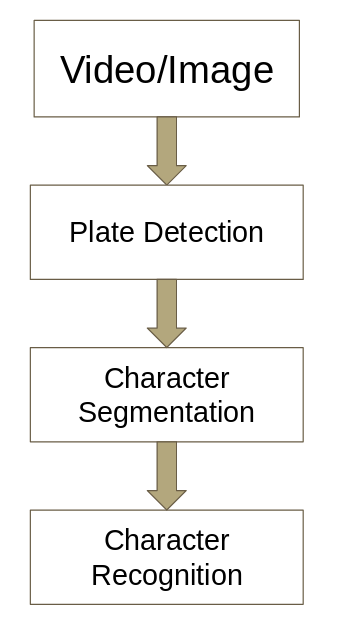
\includegraphics[width=0.8\columnwidth]{ff}
		
		\caption{
			\label{fig:samplesetup} % spaces are big no-no withing labels
			ALPR stages..
		}
		
	\end{minipage}\qquad
	\begin{minipage}[b]{.4\textwidth}
		
		\centering 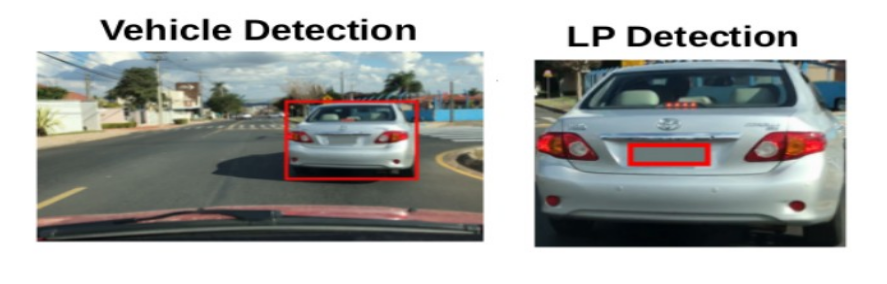
\includegraphics[width=0.8\columnwidth]{lp_detection.png}
		
		\caption{
			\label{fig:2} % spaces are big no-no withing labels
			LP Detection.
		}
		
	\end{minipage}
\end{figure*}


\section{Introduction}

In the last two decades, several highway administration companies started to perform on-track license plate recognition
on their roads. This task is commonly called Automatic License Plate Recognition (ALPR) and can be applied to achieve
multiple goals, such as stolen vehicles identification, speed traps and automatic toll collection. The importance of this
task led the research community to propose many techniques to recognize vehicles in an efficient way.

ALPR systems typically have three main stages (see figure~\ref{fig:samplesetup}).: License Plate (LP) detection, character segmentation and character recognition. The earlier stages require higher accuracy or almost perfection, since failing to detect the LP would probably lead to a failure in the next stages either. Many approaches search first for the vehicle and then its LP in order to reduce processing time and eliminate false positives.

\subsection{License Plate Detection}
This is the first and probably the most important stage of the system since failing to detect the LP would probably
lead to a failure in the next stages either. At this stage the position of the license plate (see figure~\ref{fig:2}) is determined. The input at this stage is an video frame/image of the vehicle and the output is the license plate. 

\subsubsection{Character Segmentation}
The process of identifying the characters is known as character segmentation, it is preferable to divide the extracted plate into different images (see figure~\ref{fig:3}), each containing one isolated character. There are some widely used methods for character isolation which are used in almost all available LPR systems. At this stage the characters on the license plate are mapped out and segmented into individual images. This second part of the problem, reading text, is really just a subset of the vast field of optical character recognition (OCR).


\begin{figure*}
	\centering
	\begin{minipage}[b]{.4\textwidth}
		\centering 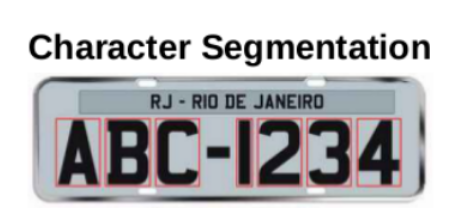
\includegraphics[width=0.8\columnwidth]{cs.png}
		
		\caption{
			\label{fig:3} % spaces are big no-no withing labels
			Character Segmentation.
		}
		
	\end{minipage}\qquad
	\begin{minipage}[b]{.4\textwidth}
		
		\centering 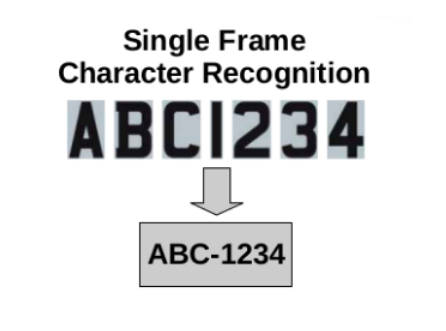
\includegraphics[width=0.8\columnwidth]{cr.png}
		
		\caption{
			\label{fig:4} % spaces are big no-no withing labels
			Character Recognition.
		}
		
	\end{minipage}
\end{figure*}



\subsubsection{Character Recognition}
This is where we wrap things up. The characters earlier segmented are identified here. We need to identify the segmented characters at this step by converting the pixel information of digital image into the ASCII text of the number plate (see figure~\ref{fig:4}).


\section{RELATED WORK}
In this section, we briefly describe some recent works in the literature that are related to the topics addressed in our work. More recently, deep learning object detectors have been employed to tackle both license plate detection (LPD) and license plate recognition (LPR). Hence, to understand previous approaches, we first need to understand the difference among
object detectors. In this section, we briefly review some recent approaches and then describe how they have been applied to
ALPR problem.

\subsection{Object Detectors based on Deep Learning}
Deep learning object detectors can be divided into two categories: one-stage and two-stage detectors. The key difference
between these two categories is how the networks obtain their region proposals. While two-stage detectors require a region
proposal network (RPN) to create candidate regions, one-stage detectors predict scores for a default set of bounding boxes,
eliminating the need for region proposal. Even though the use of two-stage detectors usually presents higher accuracy, the
required region proposal is very time consuming and prevents the use of such detectors in real scenarios. The success of one-stage detectors started with YOLO [1]. It divides the original image into a regular grid and, for each
cell, the bounding-box shape was regressed along with the confidence for each class.

\subsection{License Plate Pipeline}
In this section, we outline other deep learning techniques applied to ALPR and we also highlight on the main limitations
of previous approaches.

Silva \& Jung [2] performed both detection and recognition with the YOLO framework. The detection task was divided into car detection followed by license plate detection on each car region, which compromise its execution time. Then, YOLO was trained to detect/recognize each character on the license plate. Recently, Laroca et al. [3] improved the accuracy by separating the recognition tasks into segmentation and classification.

Hsu et al. [4] employed the YOLOv2 architecture to perform detection. As our approach, they were able to make these detections directly on the frame image without detecting a vehicle first by changing the grid and anchor boxes parameters for YOLO and YOLOv2.

\section{PROPOSED APPROACH}
In this section, we detail our proposal through the whole three main stages that we mentioned before. The proposed algorithm has been implemented for recognition of license plate characters after the processing of captured video and plate detection and can be found here \href{https://github.com/Mkamel104/ALPR }{ALPR\_gitHub link}.

\subsection{Preprocessing}
This is the first stage and at the end of this stage, we should be able to identify the license plate’s position on the car. In order to do this, we need to read the image and convert it to gray-scale. In a gray-scale image, each pixel is between 0 \& 255. We now need to convert it to a binary image in which a pixel is either complete black or white (see figure~\ref{fig:5}). After getting the frames we need to apply some preprocessing to enhance the frame, and apply some filters such as Soble (an approximation to a derivative of an image), see figure~\ref{fig:6}) and Gaussian (a linear filter, it's usually used to blur the image or to reduce noise) see figure~\ref{fig:7}). Also we need to apply Morphological transformation (operations based on the image shape.) such as opening (Opening is just another name of erosion followed by dilation). It is useful in removing noise see figure~\ref{fig:8}).



\begin{figure*}
	\centering
	\begin{minipage}[b]{.4\textwidth}
		\centering 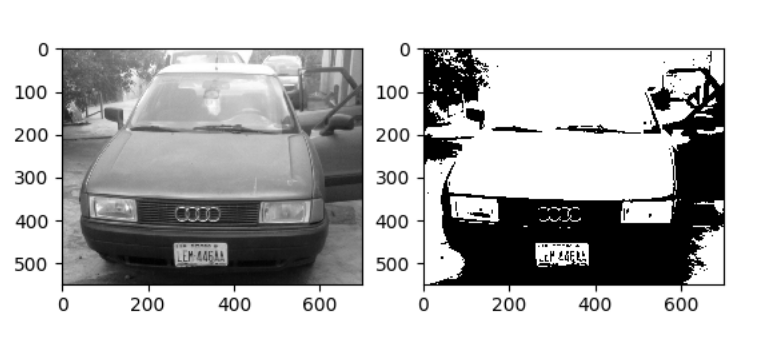
\includegraphics[width=0.8\columnwidth]{gray_binary.png}
		
		\caption{
			\label{fig:5} % spaces are big no-no withing labels
			Gray Scale \$ Binary image.
		}
		
	\end{minipage}\qquad
	\begin{minipage}[b]{.4\textwidth}
		
		\centering 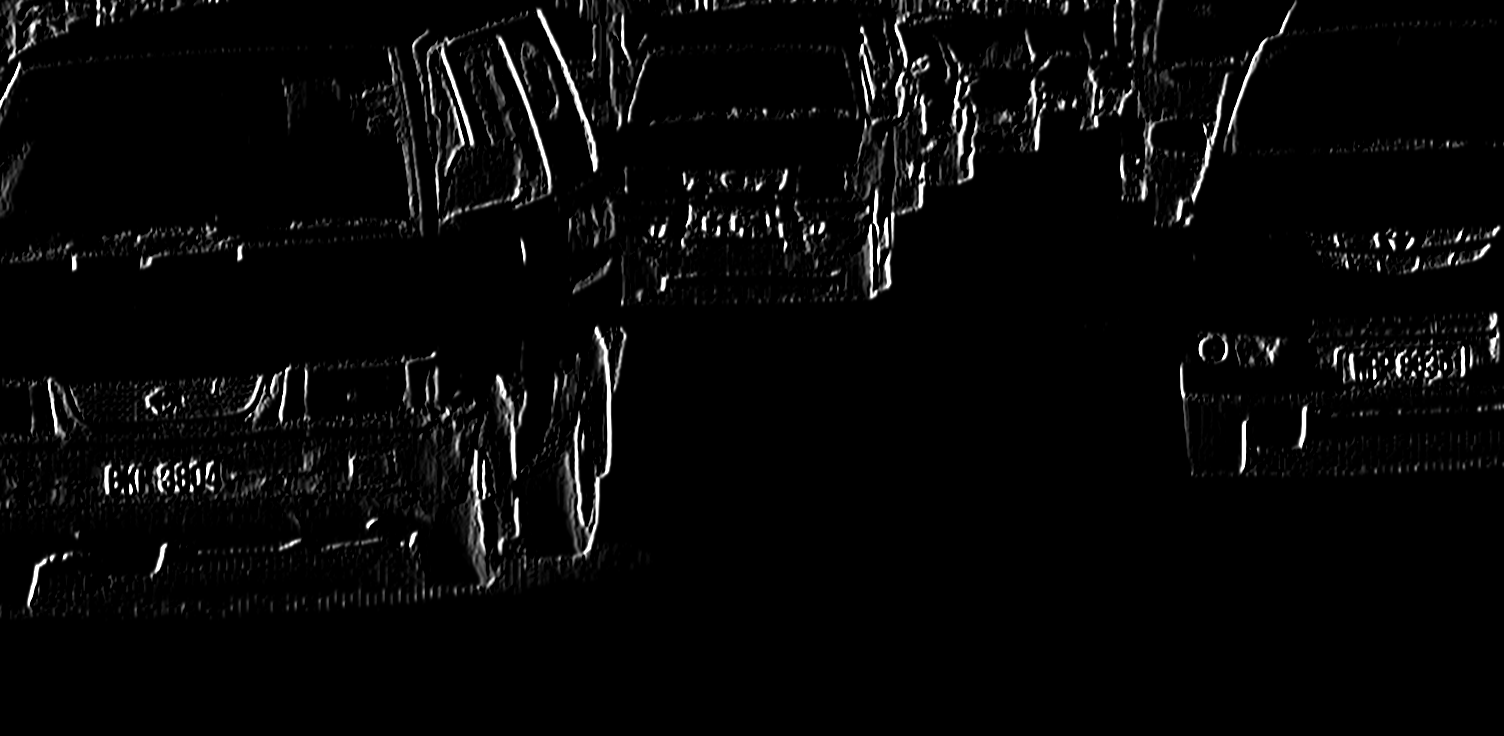
\includegraphics[width=0.8\columnwidth]{soble.png}
		
		\caption{
			\label{fig:6} % spaces are big no-no withing labels
			Soble Filter.
		}
		
	\end{minipage}
\end{figure*}


\begin{figure*}
	\centering
	\begin{minipage}[b]{.4\textwidth}
		\centering 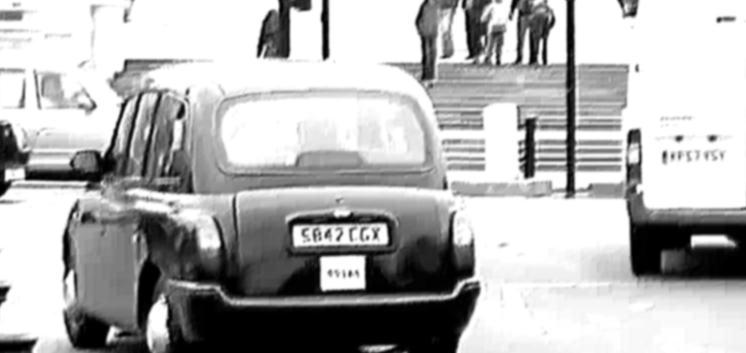
\includegraphics[width=0.8\columnwidth]{gaussian.png}
		
		\caption{
			\label{fig:7} % spaces are big no-no withing labels
			Gaussian Filter.
		}
		
	\end{minipage}\qquad
	\begin{minipage}[b]{.4\textwidth}
		
		\centering 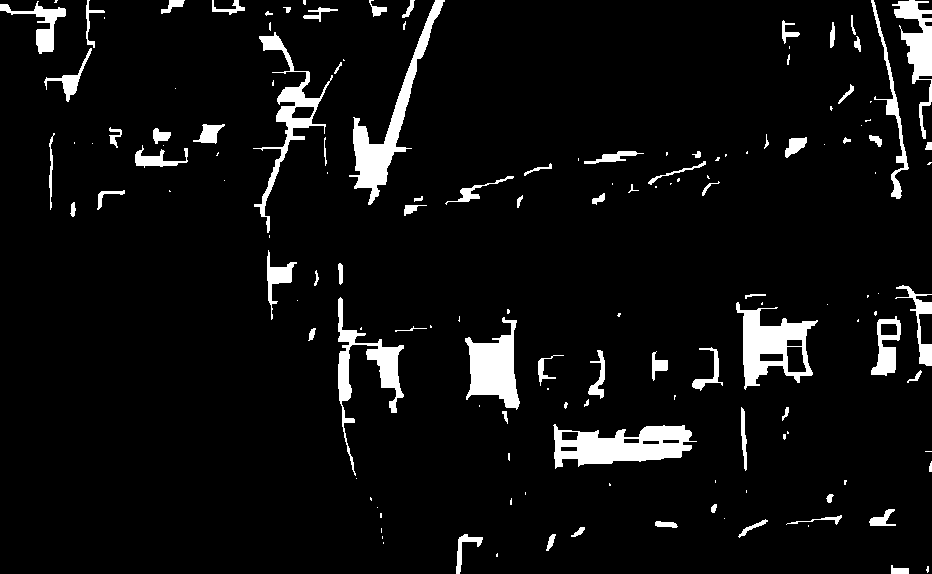
\includegraphics[width=0.8\columnwidth]{morpho.png}
		
		\caption{
			\label{fig:8} % spaces are big no-no withing labels
			Morphological transformation.
		}
		
	\end{minipage}
\end{figure*}

\begin{figure*}
	\centering
	\begin{minipage}[b]{.4\textwidth}
		\centering 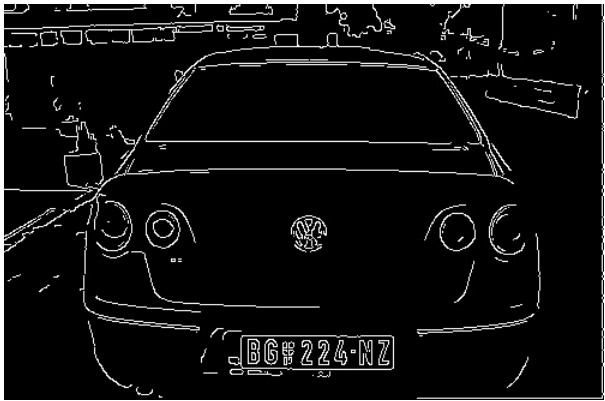
\includegraphics[width=0.8\columnwidth]{edge.png}
		
		\caption{
			\label{fig:9} % spaces are big no-no withing labels
			LP Edge finder.
		}
		
	\end{minipage}\qquad
	\begin{minipage}[b]{.4\textwidth}
		
		\centering 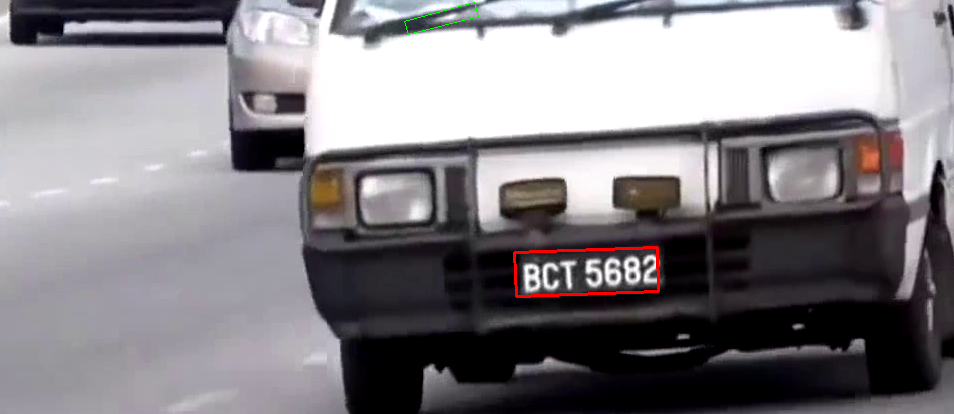
\includegraphics[width=0.8\columnwidth]{plate_detcted.png}
		
		\caption{
			\label{fig:10} % spaces are big no-no withing labels
			Actual LP detected.
		}
		
	\end{minipage}
\end{figure*}


\begin{figure*}
	\centering
	\begin{minipage}[b]{.4\textwidth}
		\centering 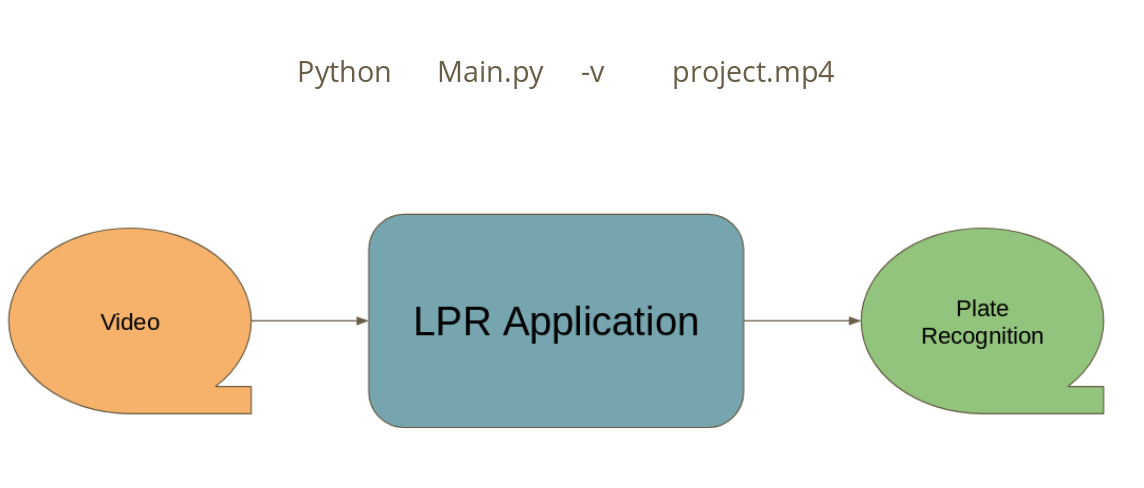
\includegraphics[width=0.8\columnwidth]{demo.png}
		
		\caption{
			\label{fig:11} % spaces are big no-no withing labels
			Demo.
		}
		
	\end{minipage}\qquad
	\begin{minipage}[b]{.4\textwidth}
		
		\centering 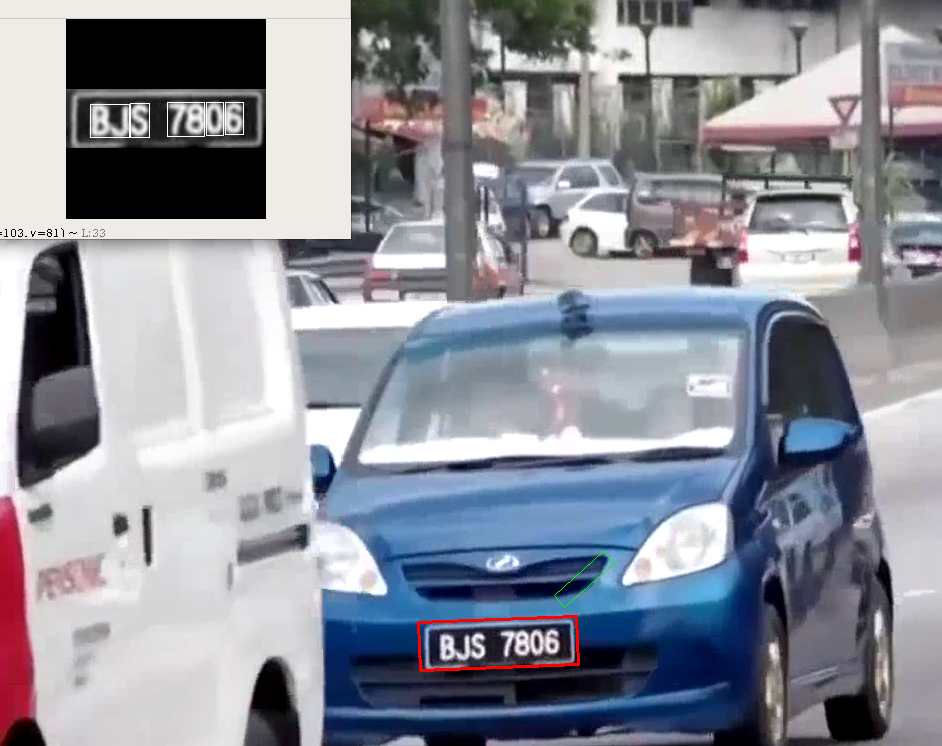
\includegraphics[width=0.8\columnwidth]{out.png}
		
		\caption{
			\label{fig:12} % spaces are big no-no withing labels
			Project Output
		}
		
	\end{minipage}
\end{figure*}


\subsection{License Plate (LP)}
For the license plate there are many different standers and we should put some characteristic for the LP that we are going to tackle in this project. 1. They are rectangular in shape. 2. The width is more than the height. 3. The proportion of the width of the license plate region to the full image ranges between 15\% and 40\%. 4. The proportion of the height of the license plate region to the full image is between 8\% \& 20\%. Also, We assume that each plate has 7 possible positions it should return a probability distribution across the 36 possible characters (26 Letters ,and 10 Numbers). (For this project I assume number plates have exactly 7 characters (letters (A-Z) and numbers (0-9)). We need to find the contours for each plate to detect it's edge see figure~\ref{fig:9}). In our project we have two colorers green(to identify the LP edge) and red (to indicate we have a plate frame that we need to process to recognize the character inside the plates) see figure~\ref{fig:10}).


\subsection{Character Segmentation}
Segmentation can be done by detecting the transition from dark to light or from light to dark level. Each character present in the number plate produces a band of gray level. So by detecting the similar gray level bands each character can be segmented. ALPR systems based on DL techniques usually address the character segmentation and recognition together. Once the LP has been detected, we employ the CNN pre-trained model for character segmentation and recognition. However, instead of performing both stages at the same time through an architecture with 36 classes (0-9, A-Z).

\subsection{Character Recognition}
This is going to be the last stage, since many characters might not be perfectly segmented, containing missing parts, and as each character is relatively small, even one pixel difference  between the ground truth and the prediction might impair the character’s recognition. Menotti et al. [5] proposed the use of random CNNs to extract features for character recognition,
achieving a significantly better performance than using image pixels or learning the filters weights with back-propagation. In this task also we used a pre-trained model using CNN.

\subsection{Experiments}
In this section, we conduct experiments to verify the effectiveness of the proposed ALPR system to work on video and real-time. To run the proposed solution just what you need is only typing one command (python Main -v $<video file>$), see figure~\ref{fig:11}). When you run our proposed algorithm you will be able to detect and recognize the LP as shown in figure~\ref{fig:12}.




\section{Conclusion and discussion}
In this project, we have presented a real-time end-to-end ALPR system using the a pre-trained CNNs models from video. After running set of experiments we found that the ALPR process depends on many factors especially when deal with video such as the position of the camera itself, quality of the video, whether, and the quality of license plate self. Definitely our project just did prove of concept to apply ALPR in real-time from video and it has a set of drawbacks like it only works with number plates in a specific format, moreover specifically, the network architecture assumes exactly 7 chars are visible in the output, in addition, it only works on specific number plate fonts.


\section{Future Work}
This project just a start in ALPR in real-time from video, and there is alot to do to enhance the this system. In this section I will try to include some ideas to enhance this system. First we need to train our own model and train it on  an existing data sets instead of using a pre-trained model. Also, We need to include different standers for different silence plates and include different languages from different countries such as Chinese letters. Furthermore, Working with different sources of videos with different resolution and trying to get the optimal model which is suitable for most cases. Finally, the output from our proposed project may be multiple frames for the same plate, so we need to apply something like majority votes to select the most correct one figure~\ref{fig:13}.


\begin{figure*}
	\centering
	\begin{minipage}[b]{.4\textwidth}
		\centering 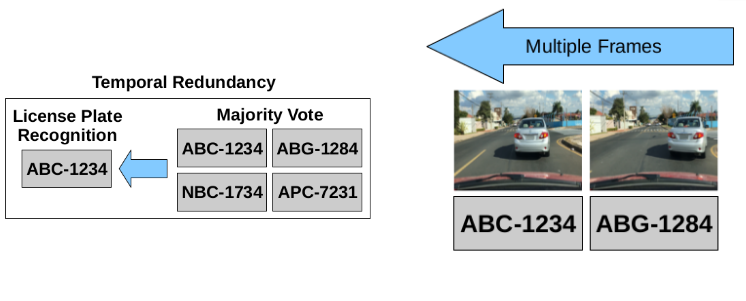
\includegraphics[width=0.8\columnwidth]{maj.png}
		
		\caption{
			\label{fig:13} % spaces are big no-no withing labels
			Multiple Frames.
		}
		
	\end{minipage}
\end{figure*}



\begin{thebibliography}{}
	
\bibitem{}	
J. Redmon, S. Divvala, R. Girshick, and A. Farhadi, “You only look
once: Unified, real-time object detection,” in Conference on Computer
Vision and Pattern Recognition (CVPR), 2016.

\bibitem{}
S. M. Silva and C. R. Jung, “Real-time brazilian license plate detection
and recognition using deep convolutional neural networks,” in Confer-
ence on Graphics, Patterns and Images (SIBGRAPI), 2017.

\bibitem{}
R. Laroca, E. Severo, L. A. Zanlorensi, L. S. Oliveira, G. R. Gonc ̧alves,
W. R. Schwartz, and D. Menotti, “A robust real-time automatic license
plate recognition based on the YOLO detector,” CoRR, 2018.

\bibitem{}
G. S. Hsu, A. Ambikapathi, S. L. Chung, and C. P. Su, “Robust license
plate detection in the wild,” in International Conference on Advanced
Video and Signal Based Surveillance (AVSS), 2017.


\bibitem{}
D. Menotti, G. Chiachia, A. X. Falc ̃ao, and V. J. O. Neto, “Vehicle
license plate recognition with random convolutional networks,” in 2014
27th SIBGRAPI Conference on Graphics, Patterns and Images, Aug
2014, pp. 298–303.

\bibitem{}
\href{http://www.anpr.net/}{ANPR}
\bibitem{}
\href{http://www.licenseplaterecognition.com/}{license plate recognition}

\bibitem{}
\href{https://matthewearl.github.io/2016/05/06/cnn-anpr/}{Deep ALPR}
 


\end{thebibliography}


\end{document}
